\documentclass[12pt]{article}
%\usepackage{natbib}
\usepackage[french]{babel}
\usepackage{url}
\usepackage[utf8x]{inputenc}
\usepackage{graphicx}
\graphicspath{{images/}}
\usepackage{parskip}
\usepackage{fancyhdr}
\usepackage{vmargin}
\usepackage{xcolor}
\usepackage{bbm}
\usepackage{amsmath,amssymb}
\usepackage{amsthm}
\usepackage{dsfont}
\usepackage{stmaryrd}
\usepackage{systeme}
\usepackage{enumitem}
\usepackage{xcolor}
\usepackage{pifont}
\usepackage{textcomp}
\usepackage{calrsfs}
\usepackage{listings}


\definecolor{darkWhite}{rgb}{0.94,0.94,0.94}
 
\lstset{%
  language=Python,
  basicstyle   = \ttfamily,
  keywordstyle =    \color{magenta},
  keywordstyle = [2]\color{orange},
  commentstyle =    \color{gray}\itshape,
  stringstyle  =    \color{cyan},
  literate=
  {²}{{\textsuperscript{2}}}1
  {⁴}{{\textsuperscript{4}}}1
  {⁶}{{\textsuperscript{6}}}1
  {⁸}{{\textsuperscript{8}}}1
  {€}{{\euro{}}}1
  {é}{{\'e}}1
  {è}{{\`{e}}}1
  {ê}{{\^{e}}}1
  {ë}{{\¨{e}}}1
  {É}{{\'{E}}}1
  {Ê}{{\^{E}}}1
  {û}{{\^{u}}}1
  {ù}{{\`{u}}}1
  {â}{{\^{a}}}1
  {à}{{\`{a}}}1
  {á}{{\'{a}}}1
  {ã}{{\~{a}}}1
  {Á}{{\'{A}}}1
  {Â}{{\^{A}}}1
  {Ã}{{\~{A}}}1
  {ç}{{\c{c}}}1
  {Ç}{{\c{C}}}1
  {õ}{{\~{o}}}1
  {ó}{{\'{o}}}1
  {ô}{{\^{o}}}1
  {Õ}{{\~{O}}}1
  {Ó}{{\'{O}}}1
  {Ô}{{\^{O}}}1
  {î}{{\^{i}}}1
  {Î}{{\^{I}}}1
  {í}{{\'{i}}}1
  {Í}{{\~{Í}}}1,
  aboveskip=3mm,
  belowskip=-2mm,
  backgroundcolor=\color{darkWhite},
  breaklines=true,
   showspaces=false,
  showstringspaces=false,
  showtabs=false,
}


\title{Rapport Projet}
\author{BRANDEL Clément, CARVAILLO Thomas, PONS Hugo}
\date{\today}

\makeatletter
\let\thetitle\@title
\let\theauthor\@author
\let\thedate\@date
\makeatother

\pagestyle{fancy}
\fancyhf{}
\rhead{\theauthor}
\lhead{\thetitle}
\cfoot{\thepage}
\def\dotfill#1{\cleaders\hbox to #1{.}\hfill}
\newcommand\dotline[2][.5em]{\leavevmode\hbox to #2{\dotfill{#1}\hfil}}



\newcommand{\R}{\mathbbm{R}}
\newcommand{\N}{\mathbbm{N}}
\newcommand{\1}{\mathbbm{1}}
\newcommand{\E}{\mathbbm{E}}
\newcommand{\V}{\mathbbm{V}}
\newcommand{\Prob}{\mathbbm{P}}
\newcommand{\Nc}{\mathcal{N}}
\newcommand{\Cc}{\mathcal{C}}
\newcommand{\Xti}{\widetilde{X_i}}
\newcommand{\Xtj}{\widetilde{X_j}}
\newcommand{\Xn}{\overline{X_n}}
\newcommand{\gn}{\hat{g_n}}

%définition commande présentation fonction
\newcommand{\fonction}[5]{
\begin{displaymath}
\begin{array}{l|rcl}
\displaystyle
#1 : & #2 & \longrightarrow & #3 \\
    & #4 & \longmapsto & #5
\end{array}
\end{displaymath}
}
%fin définition

% de jolies accolades
\newcommand{\accolade}[2]{
\begin{displaymath}
%#1 = \left\{
    \begin{array}{ll}
       #1 %& \mbox{si }
       #2 %& \mbox{sinon.}
    \end{array}
\right.
\end{displaymath}
}
% de jolies accolades





\begin{document}

%%%%%%%%%%%%%%%%%%%%%%%%%%%%%%%%%%%%%%%%%%%%%%%%%%%%%%%%%%%%%%%%%%%%%%%%%%%%%%%%%%%%%%%%%

\begin{titlepage}
	\centering
    \vspace*{0.5 cm}
    \textsc{\LARGE Sécurité des Usages TIC}\\[1.0 cm]
	\vspace{1.5cm}
	\rule{\linewidth}{0.2 mm} \\[0.4 cm]
	{ \huge \bfseries  \thetitle}\\ %\color{blue}
	\rule{\linewidth}{0.2 mm} \\[1.5 cm]
	
	\begin{minipage}{0.4\textwidth}
		\begin{flushleft} \large
			\emph{A l'attention de :}\\
			Pierre François Bonnefoi\\
			\phantom{a}\\
			\phantom{a}\\
		\end{flushleft}
	\end{minipage}
	\begin{minipage}{0.5\textwidth}
    	\begin{flushright} \large
		\emph{Rédigé par :}\\
		BRANDEL Clément \\
		CARVAILLO Thomas \\
		PONS Hugo \\
		\end{flushright}
	\end{minipage}\\[2 cm]
\end{titlepage}

%%%%%%%%%%%%%%%%%%%%%%%%%%%%%%%%%%%%%%%%%%%%%%%%%%%%%%%%%%%%%%%%%%%%%%%%%%%%%%%%%%%%%

\tableofcontents
\vspace{1cm}

\section{Préambule}
Il est nécessaire d'exécuter les programmes dans un ordre spécifique:

\begin{enumerate}
{\large	
	\item Serveur.py
	\item \textit{Facultatif:} cast la comande socat dans le terminal
	\item FaciliteurDesRequêtes.py ou FaciliteurAvecSocat.py suivant 2)
}
\end{enumerate}



\pagebreak


%%%%%%%%%%%%%%%%%%%%%%%%%%%%%%%%%%%%%%%%%%%%%%%%%%%%%%%%%%%%%%%%%%%%%%%%%%%%%%%%%%%%%



%%%%%%%%%%%%%%%%%%%%%%%%%%%%%%%%%%%%%%%%%%%%%%%%%%%%%%%%%%%%%%%%%%%%%%%%%%%%%%%%%%%%%

\section{Explicitation du code}

Nous expliquerons ici les principales fonctions du projet, à savoir celles contenues dans le fichier \textit{Serveur.py}

\subsection{fonction \textit{création$\_$attestation()}}

\begin{enumerate}[label=(\arabic*)]

\item La première étape consiste en la récupération du nom, du prénom et de l'intitulé de la certification

\begin{lstlisting}
contenu_intitulé_certification = request.forms.get('certitule')

contenu_identité = request.forms.get('identite')	

cmd1='texte_attestation="'+str(contenu_intitulé_certification)+'|Attestation de réussite|délivrée à:|'+str(contenu_identité)+'" && curl -o texte.png "http://chart.apis.google.com/chart" --data-urlencode "chst=d_text_outline" --data-urlencode "chld=000000|56|h|FFFFFF|b|${texte_attestation}"'

c_line1 = "echo "+str(contenu_identité)+str(contenu_intitulé_certification)+" > texte.txt"
\end{lstlisting}
\vspace*{7mm}
La récupération du nom, prénom ainsi que l'intitulé de certification ce fait automatiquement lors de l'utilisation de la requète curl. Ensuite, à l'aide des informations récupéré on créé une image contenant le texte. Par ailleurs, on insère les informations dans un fichier texte

\item Création de l'image : 

\begin{itemize}
		\item fond de l'attestation 
		\item intégration du QRcode ($\#$1 contenant la sign [ASCII] ) $\Rightarrow$ $\#$2 création du Qrcode 	
		\item intégration du texte Nom, Prénom et Intitulé Certif
\end{itemize}	

Pour intégrer chacunes des images dans l'image final, nous utilisons les commandes de ImageMagick : 

\begin{lstlisting}
redim =subprocess.Popen('mogrify -resize 1000x600 texte.png',shell=True,stdout=subprocess.PIPE)
	
redim2 =subprocess.Popen('mogrify -resize 220x220 qrcode.png',shell=True,stdout=subprocess.PIPE)
	
fusion1 =subprocess.Popen('composite -gravity center texte.png fond_attestation.png combinaison.png',shell=True,stdin = subprocess.PIPE,stdout=subprocess.PIPE)
	
fusion2=subprocess.Popen('composite -geometry +1418+934 qrcode.png combinaison.png attest.png',shell=True,stdin = subprocess.PIPE,stdout=subprocess.PIPE)
\end{lstlisting}		
\vspace*{7mm}
\item La troisième étape est la construction du bloc d'informations (nom, prénom, ...)

\begin{lstlisting}
bloc_info = str(contenu_identité)+str(contenu_intitulé_certification)
\end{lstlisting}
\vspace*{7mm}
Le bloc d'information est une chaîne de caractères comprenant le nom, prénom et l'intitulé de certication

\item On ajoute ensuite un \textit{time stamp} dans le bloc d'informations. Pour la création du timestamp, il faut utiliser deux commandes. 

\begin{lstlisting}
c_line1 = "openssl ts -query -data "+nom_fichier+" -no_nonce -sha256 -out "+nom_fichier+".tsq"
 
c_line2 = "curl -H 'Content-Type: application/timestamp-query' --data-binary '@"+nom_fichier+".tsq' https://freetsa.org/tsr > "+nom_fichier+".tsr"
\end{lstlisting}
\vspace*{7mm}
La première commande permet de générer un fichier \textit{TimeStampRequest} et la seconde commande envoie une requête afin d'obtenir un TimeStamp à partir du \textit{TimeStampRequest}. Ensuite on convertit le contenu du TimeStamp en base64 puis on l'ajoute au bloc d'informations à dissumuler.

\begin{lstlisting}
timestamp = 'texte.txt.tsr'
timestamp = fichier_vers_Variable64(timestamp) #timestamp en base64
Message = ajoutCaractère(bloc_info,64)+timestamp # taille  = 64 + 1828
\end{lstlisting}
\vspace*{7mm}
\item Une cinquième étape consiste en la dissimulation par Stéganographie \newline
La dissimulation des informations se réalise à l'aide des fonctions données dans l'énoncé du sujet.

\item

\begin{enumerate}[label=(\roman*)]
\item On réalise la création de la signature
\begin{lstlisting}
c_line2 = "openssl dgst -sha256 -sign ecc.ca.kpriv.pem -passin pass:password texte.txt | base64" 
	
cmd2 = subprocess.Popen(c_line2,shell=True,stdin=subprocess.PIPE,stdout=subprocess.PIPE)
(data, ignorer) = cmd2.communicate()	

data = data.decode()[:-2]

datASCII=[ord(c) for c in data]
\end{lstlisting}
\vspace*{7mm}
Pour effectuer une signature sur un fichier, il suffit d'une clé privée et d'un fichier à signer. Par ailleurs, la clé privée étant sécurisé par un chiffrement AES, il est nécessaire d'intégrer le mot de passe de la clé dans la commande. Dans notre cas, on convertit directement le contenu de la signature en base64 afin de pouvoir le convertir en ASCII.

\item On crée un Qrcode contenant et la signature et la clé privée.
\end{enumerate}

\begin{lstlisting}
qr=qrcode.make(datASCII)
qr.save(nomqr,scale=2)
\end{lstlisting}	
\vspace*{7mm}
La création du Qrcode se fait en important le module \textit{qrcode}. Dans notre cas, on créé un Qrcode contenant la signature réalisée ci-dessus. 
	
\end{enumerate}

	
\subsection{fonction \textit{vérification$\_$attestation()}}

\begin{enumerate}[label=(\arabic*)]	
	
\item En premier lieu, on récupère l'image envoyée par le \textit{curl} et on en crée une copie que l'on pourra ensuite éditer et utiliser à loisir pour compléter notre vérification. 

\begin{lstlisting}
contenu_image = request.files.get('image')

contenu_image.save('attestation_a_verifier.png',overwrite=True)

response.set_header('Content-type', 'text/plain')

image=Image.open('attestation_a_verifier.png')
\end{lstlisting}
\vspace*{7mm}
\item Pour la suite, on commence par récupérer l'ensemble du message caché par stéganographie dans l'attestation. On connait déjà la taille du message à récupérer puisque lors de la création on a fait en sorte qu'il fasse 1892 caractères (64+1828). On récupère ensuite les informations du titulaire de l'attestation, i.e. son nom, prénom et intitulé de certification, que l'on stocke ensuite dans un fichier texte.

\begin{lstlisting}
MessStegano=recuperer(image, 1892)
nminti=''
g=0
while MessStegano[g] != '+':
	nminti += MessStegano[g]
	g+=1
cmd7='echo "'+nminti+'" > texte.txt'
h=subprocess.Popen(cmd7,shell=True,stdin=subprocess.PIPE,stdout=subprocess.PIPE)
\end{lstlisting}
\vspace*{7mm}

\item Pour le traitement du QRcode on va d'abord créer un .png contenant l'attestation rognée pour qu'il ne contienne que le QRcode.

\begin{lstlisting}
cmd5='convert attestation_a_verifier.png -crop 220x220+1418+934 qrcodeA.png'

prqr=subprocess.Popen(cmd5,shell=True,stdin=subprocess.PIPE,stdout=subprocess.PIPE)
time.sleep(1)

qrcrop = Image.open("qrcodeA.png")

data2 =zbarlight.scan_codes(['qrcode'],qrcrop) # début traitement QRCODE

qrcrop.close()
\end{lstlisting}
\vspace*{7mm}

\item Il nous faut faire plusieurs traitements à la donnée récupérée par le \textit{scan$\_$codes} pour retrouver la signature mise dans l'attestation dans un string. Une fois cela fait, on la décode, puis la stocke dans une fichier signature que l'on peut ensuite vérifier avec la commande \textit{openssl dgst} et notre clé publique. On récupère le résultat de cette vérification avec le \textit{.communicate()} et on le garde dans \textit{QRVERIF}.

\begin{lstlisting}
data3=data2[0].decode()
ldt=list(data3)
ldt.pop(0)
ldt.pop(len(ldt)-1)
data4=''

for x in range(0,len(ldt)):
	data4=data4+ldt[x]
dataf=data4.split(',')

for y in range(0,len(dataf)):
	dataf[y]=int(dataf[y])
dataQRCODE=''

for z in range(0,len(dataf)):
	dataQRCODE=dataQRCODE+chr(dataf[z]) 
	dataQRCODE += '='
	
c_line3 = "echo '"+dataQRCODE+"' | base64 -d > signature.sign.bin"

cmd4 = subprocess.Popen(c_line3,shell=True,stdin=subprocess.PIPE,stdout=subprocess.PIPE)
time.sleep(0.2)

cmd6='openssl dgst -sha256 -verify ecc.ca.kpub.pem -signature signature.sign.bin texte.txt'

i=subprocess.Popen(cmd6,shell=True,stdin=subprocess.PIPE,stdout=subprocess.PIPE)
(retour,ignorer)=i.communicate()

QRVERIF=retour.decode()
\end{lstlisting}
\vspace*{7mm}
\item Il reste à vérifier le \textit{timestamp} se trouvant dans le message stéganographié, il compose les 1828 derniers caractères du message. Après l'avoir décodé on crée un fichier le contenant, que l'on utilise finalement pour vérifier le timestamp. Le résultat est récupéré et stocké dans \textit{TIMESTAMPVERIF}.

\begin{lstlisting}
Tsp=MessStegano[64:]+'='
cmd8='echo "'+Tsp+'" | base64 -d > texte.txt.tsr'

k=subprocess.Popen(cmd8,shell=True,stdin=subprocess.PIPE,stdout=subprocess.PIPE)
time.sleep(0.2)

cmd9='openssl ts -verify -data texte.txt -in texte.txt.tsr -CAfile cacert.pem -untrusted tsa.crt'

l=subprocess.Popen(cmd9,shell=True,stdin=subprocess.PIPE,stdout=subprocess.PIPE)

(revers,ignorer)=l.communicate()
TIMESTAMPVERIF=revers.decode()
\end{lstlisting}
\vspace*{7mm}	

\item On vérifie finalement que 
\begin{lstlisting}
QRVERIF == 'Verified OK\n' 
\end{lstlisting}
\vspace*{7mm}
et 
\begin{lstlisting}
TIMESTAMPVERIF == 'Verification: OK\n' 
\end{lstlisting}
\vspace*{7mm}
et si ces deux conditions sont satisfaites, alors l'attestation est bel et bien authentique.

\end{enumerate}




%%%%%%%%%%%%%%%%%%%%%%%%%%%%%%%%%%%%%%%%%%%%%%%%%%%%%%%%%%%%%%%%%%%%%%%%%%%%%%%%%%%%%
\pagebreak

\section{Exemple d'exécution}

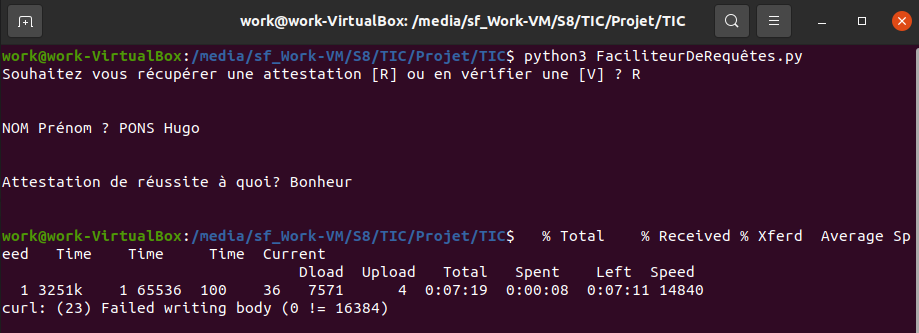
\includegraphics[scale=0.5]{img1.png}
\newline
\break
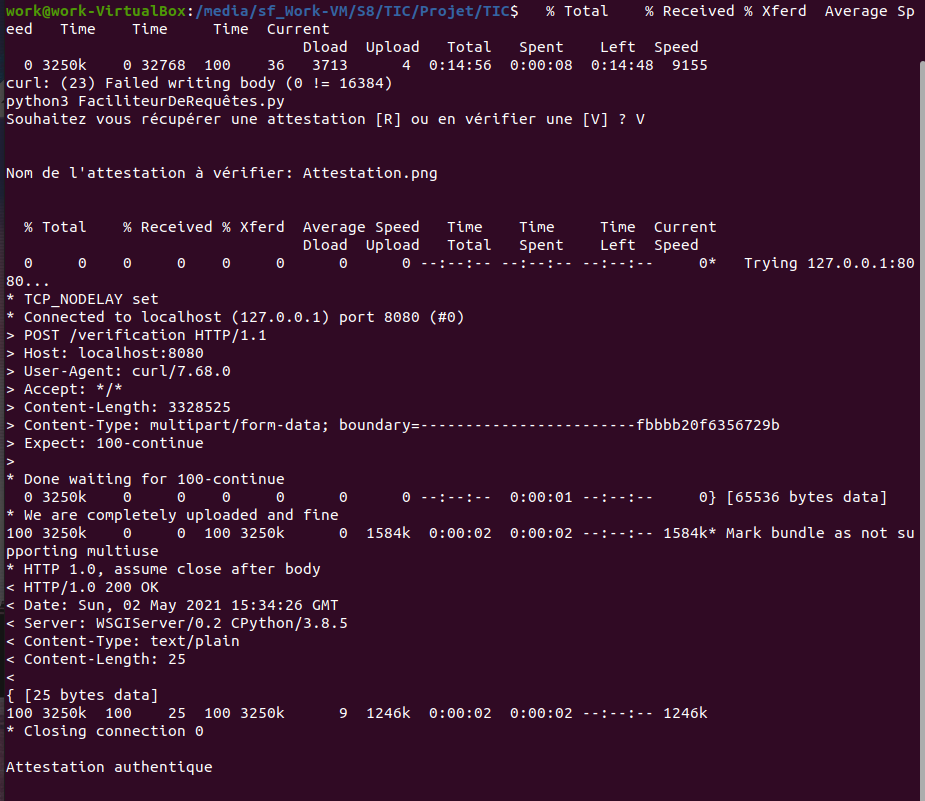
\includegraphics[scale=0.5]{img2.png}
\newline
\break
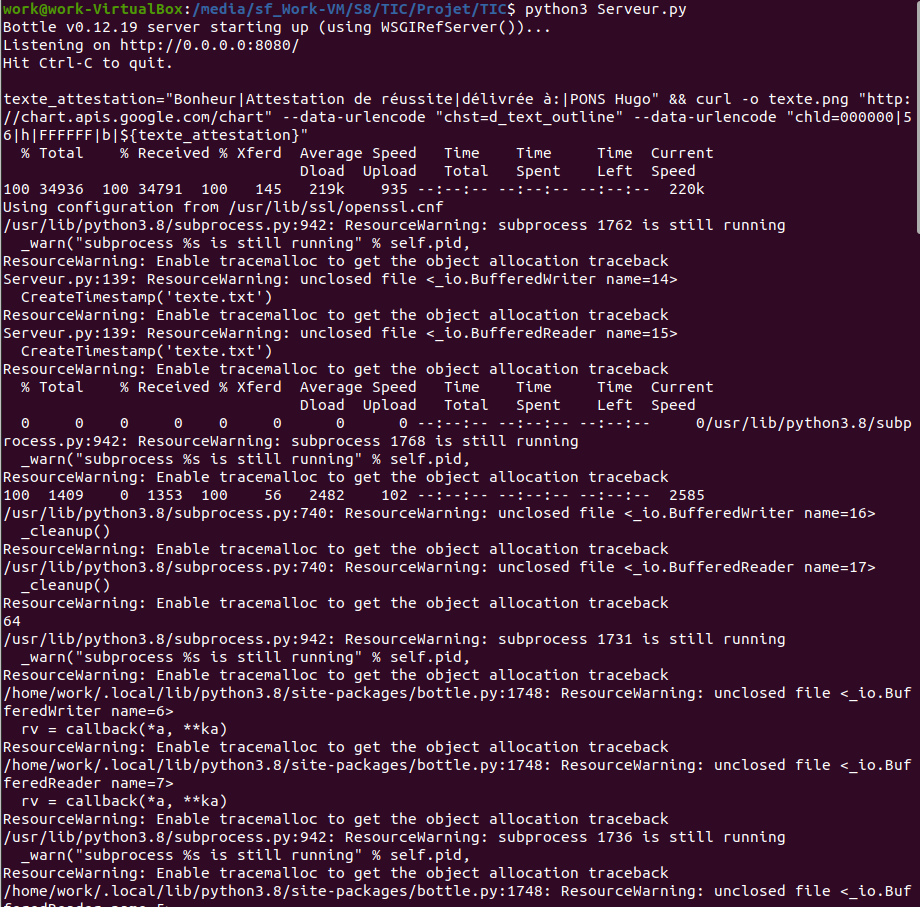
\includegraphics[scale=0.5]{img3.png}


%%%%%%%%%%%%%%%%%%%%%%%%%%%%%%%%%%%%%%%%%%%%%%%%%%%%%%%%%%%%%%%%%%%%%%%%%%%%%%%%%%%%%








%\addcontentsline{toc}{part}{Références}

%\begin{thebibliography}{9}
	%\bibitem{these1}
	%Référence 1
%\end{thebibliography}

\end{document}
